\subsection{Diagrammi UML comportamentali}
In questa sezione sono riportati alcuni diagrammi comportamentali a corredo dei diagrammi dei casi d'uso e UML delle classi che illustrano il funzionamento della seconda versione dell'applicazione.

I diagrammi UML riportati di seguito sono altamente descrittivi, in modo da essere utilizzabili per mostrare all'utente in maniera intuitiva il funzionamento dell'applicazione, pur rispettando le direttive UML.\bigskip

\newpage
\textbf{Diagramma degli Stati: Ciclo di vita dell'utente Configuratore}\newline
In Figura \ref{fig:State diagram 2.1} è rappresentato il ciclo di vita dell'utente Configuratore: a seconda dell'azione che esso intraprende nei confronti dell'applicazione il Configuratore si trova in un determinato stato.\newline L'accesso all'applicazione può avvenire o in qualità di primo accesso oppure come accesso ordinario: nel caso si tratti di un primo accesso il configuratore si riconduce allo stato \texttt{CreazioneProfilo} in cui avviene la creazione di un nuovo profilo Configuratore a cui segue un necessario cambio delle credenziali, mentre nel caso si tratti di un login ordinario l'utente accede direttamente al menu principale. \newline 
In tutti i passaggi di stato si considera la situazione ideale in cui non vi siano errori nell'esecuzione delle operazioni. Nel caso in cui si verifichino errori di esecuzione allora è lasciato sottinteso il passaggio attraverso uno stato di Errore prima di tornare al menu principale.

\begin{figure}[!]
\centering
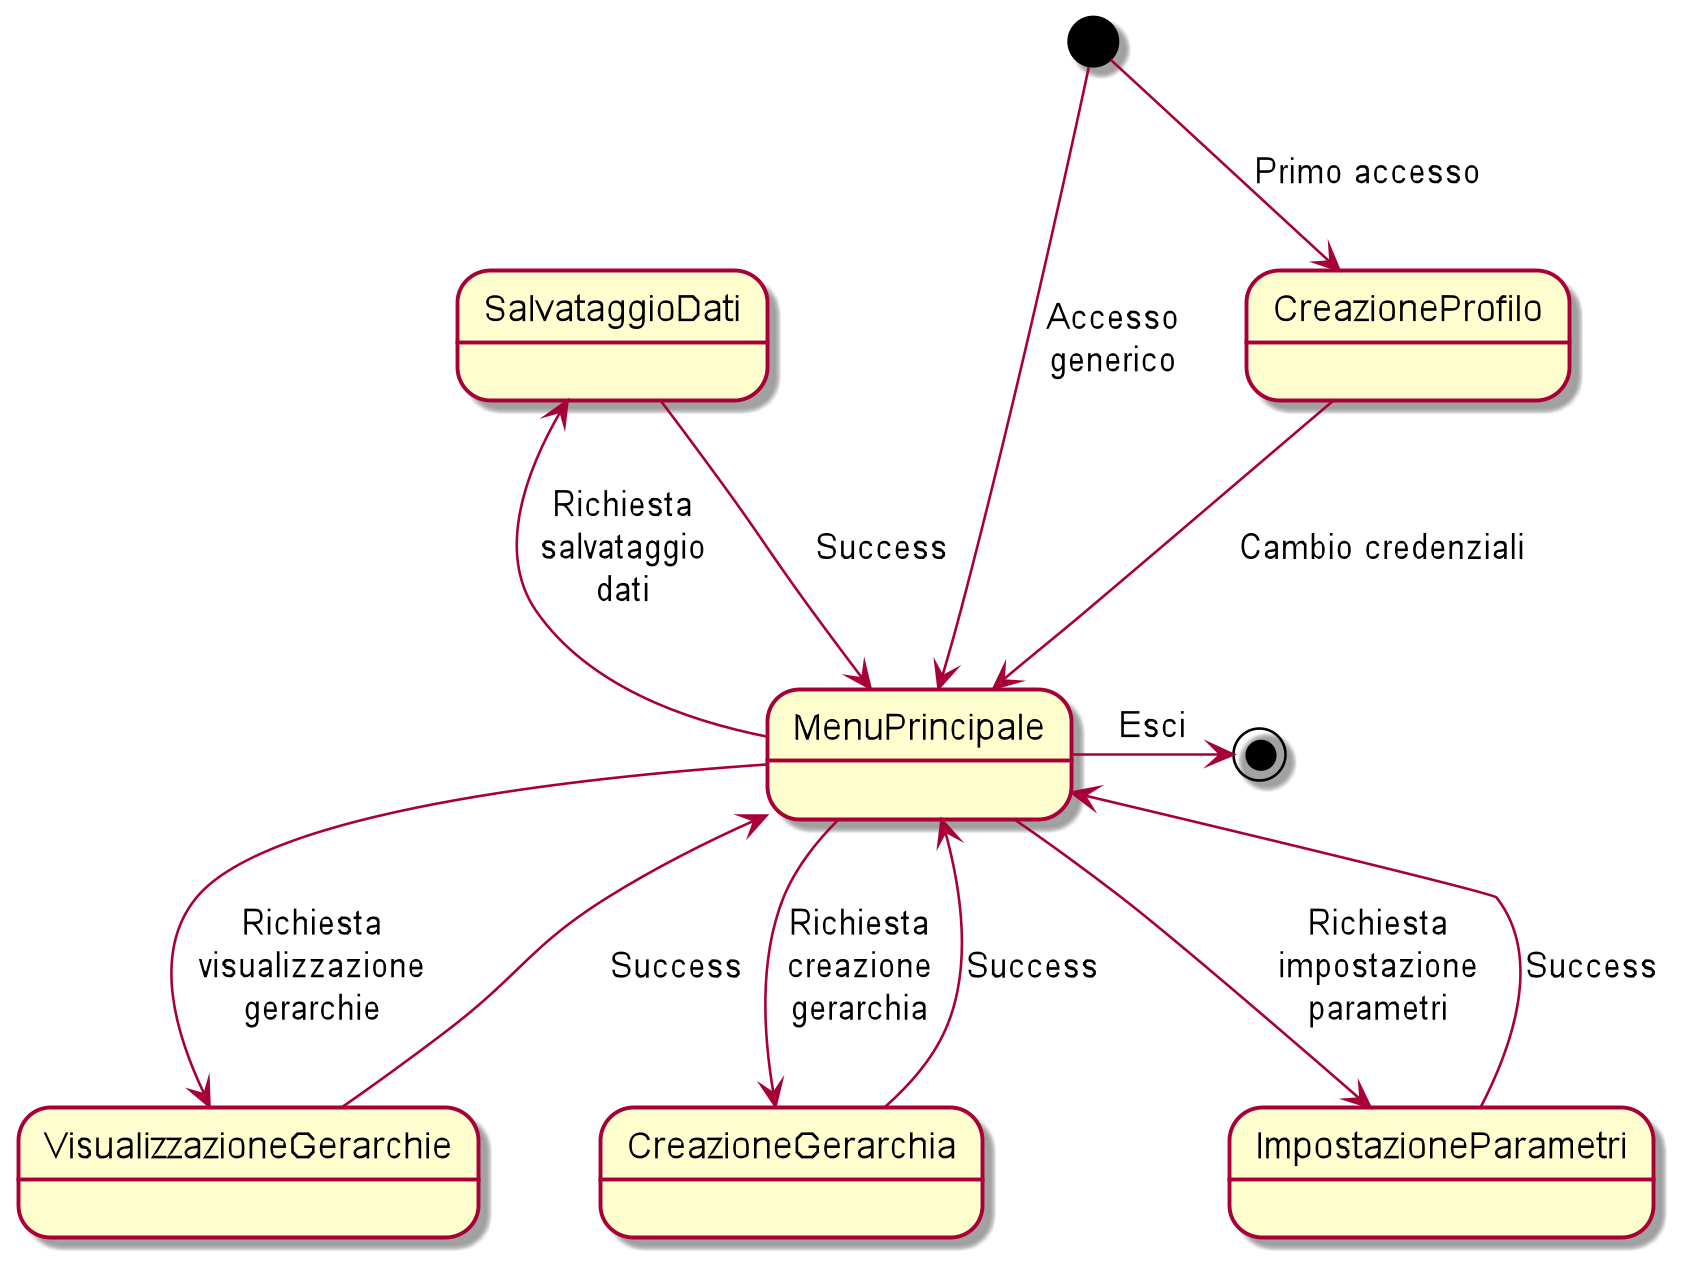
\includegraphics[width=0.7\textwidth]{imagesV2/State diagram-interazione configuratore v2.png}
\caption{\label{fig:State diagram 2.1}Ciclo di vita del Configuratore - Versione 2}
\end{figure}\bigskip

\textbf{Diagramma degli Stati: Ciclo di vita dell'utente Fruitore}\newline
In Figura \ref{fig:State diagram 2.2} è rappresentato il ciclo di vita dell'utente Fruitore: a seconda dell'azione che esso intraprende nei confronti dell'applicazione il Fruitore si trova in un determinato stato.\newline L'accesso all'applicazione può avvenire o in qualità di primo accesso oppure come accesso ordinario: nel caso si tratti di un primo accesso il Fruitore si riconduce allo stato \texttt{CreazioneProfilo} in cui avviene la creazione di un nuovo profilo Fruitore, mentre nel caso si tratti di un login ordinario l'utente accede direttamente al menu principale. \newline 
In tutti i passaggi di stato si considera la situazione ideale in cui non vi siano errori nell'esecuzione delle operazioni. Nel caso in cui si verifichino errori di esecuzione allora è lasciato sottinteso il passaggio attraverso uno stato di Errore prima di tornare al menu principale.

\begin{figure}[!]
\centering
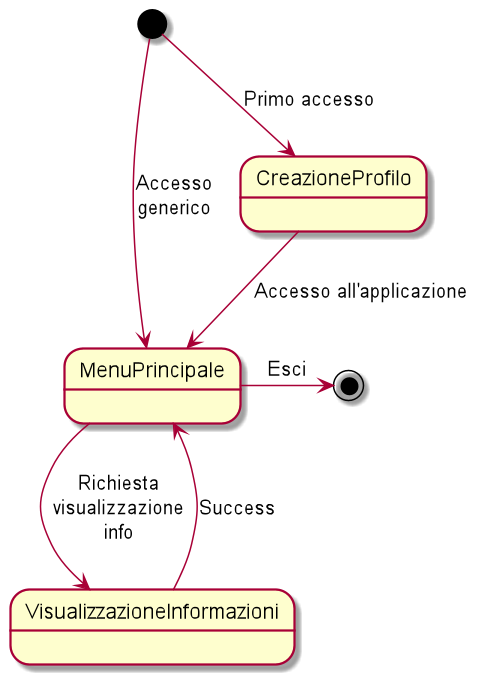
\includegraphics[width=0.5\textwidth]{imagesV2/State diagram-interazione fruitore v2.png}
\caption{\label{fig:State diagram 2.2}Ciclo di vita del Fruitore - Versione 2}
\end{figure}\bigskip